\newpage
\chapter{Hardware}

\section{Schmetic}
På figur \ref{fig:schematics} ses tegning over hardware setup. \textit{Signal in}, \textit{Signal out(A3)} og \textit{Signal out(A4)} skal ses som interface med arduino og tryksensoren. Disse er undladt for ikke gøre diagrammet for kompleks
\begin{figure}[H]
	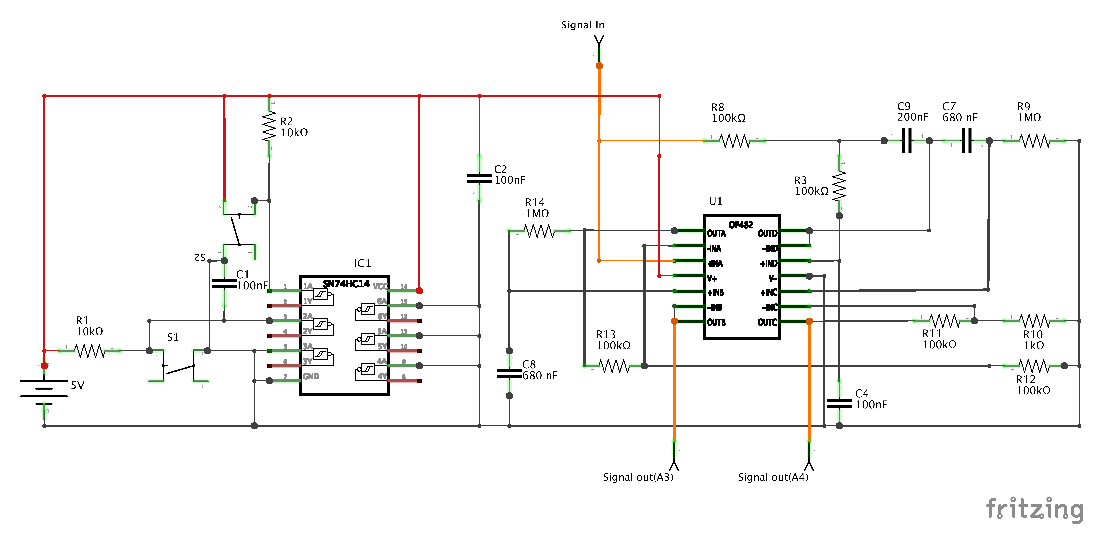
\includegraphics[trim = 0 30 0 0, clip=true, width = \textwidth]{billeder/Konditionering_schem.pdf}
	\caption{}\label{fig:schematics}
\end{figure}

\newpage
\section{Knapper} \label{title:buttons}
For at imødegå debouncing ved tryk på knapperne, er der bygget et støttekredsløbs til disse. Debouncing kan ses på figur \ref{fig:withbounce} hvor det mekaniske slip på knappen, giver anledning til en løs forbindelse ses på multimeteret som en lav efterfulgt af en høj, for så at blive lav igen. Microcontrolleren er hurtig nok til at registrer dette som et nyt knaptryk.
\begin{figure}[H]
	\begin{minipage}{0.50\textwidth}
		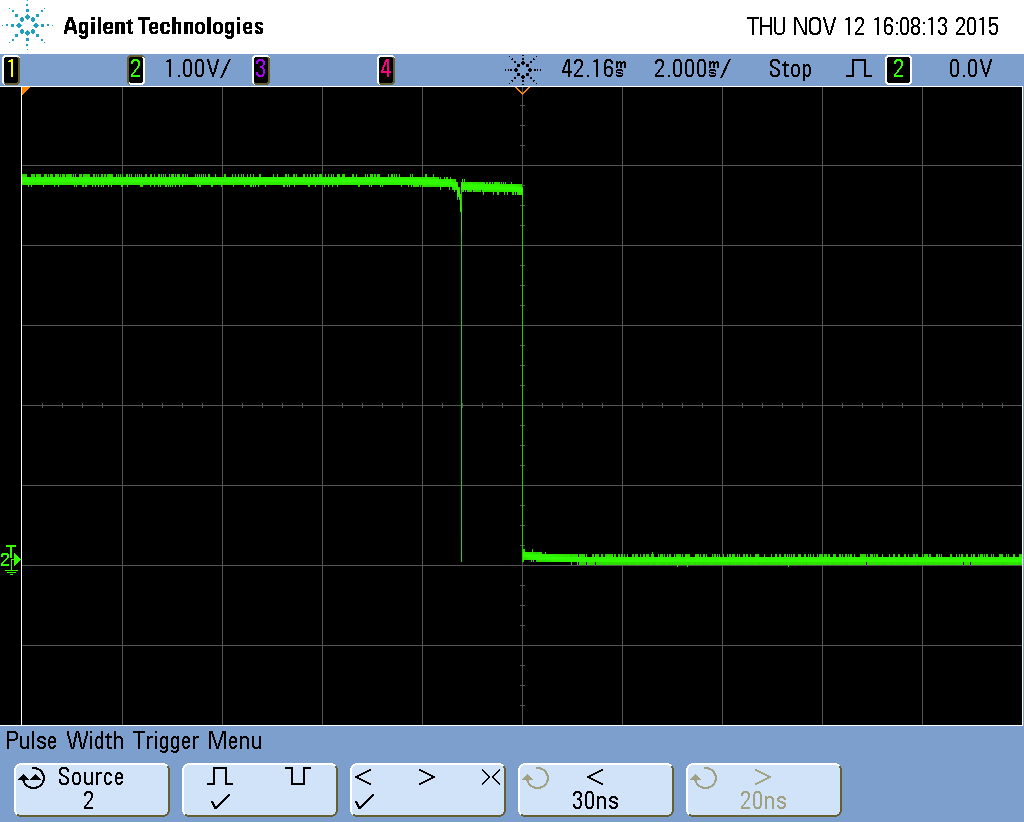
\includegraphics[width = \textwidth]{billeder/scope_14.png}
		\caption{Figuren viser et knaptryk, hvor der opstår debouncing.}\label{fig:withbounce}
	\end{minipage}
	\begin{minipage}{0.50\textwidth}
		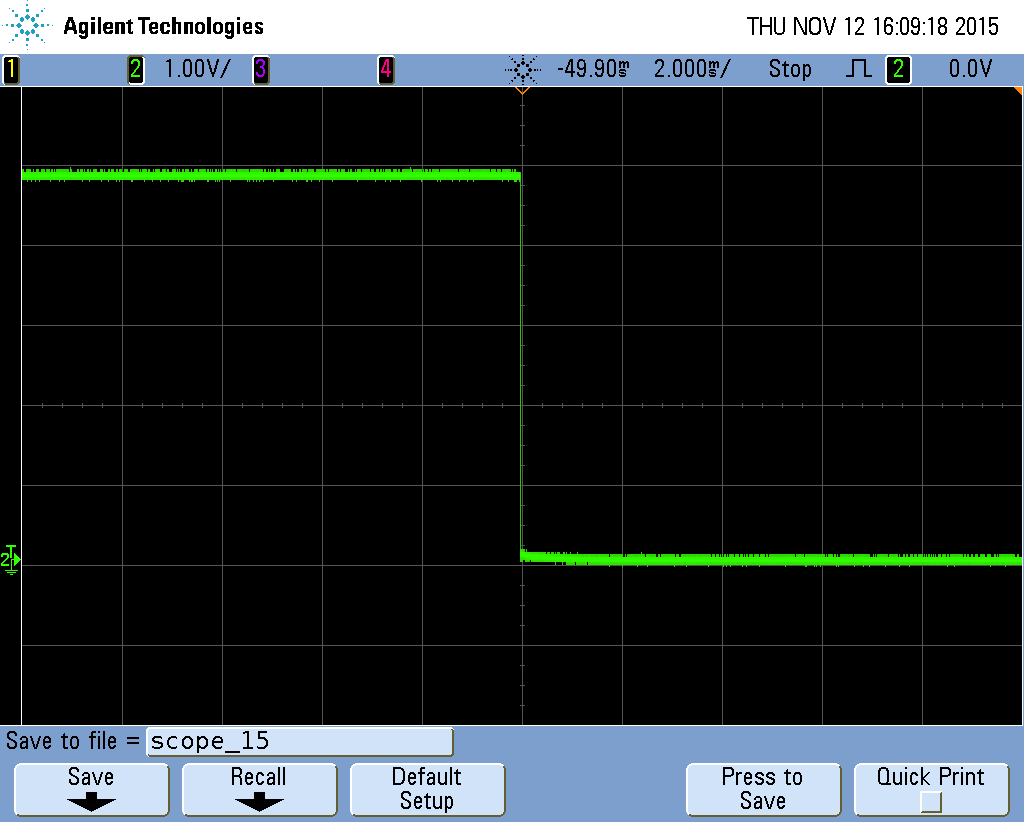
\includegraphics[width = \textwidth]{billeder/scope_15.png}
		\caption{Knaptryk hvor der er implementeret et anti debouncing kredsløb.}\label{fig:withoutbounce}
	\end{minipage}
\end{figure}

For at imødekomme  er der implementeret et debounce kredsløb (figur \ref{fig:antidebouncingcircuit}) med en inverting schmitt trigger. Schmitt triggeren leverer en stabil høj og kapacitoren forhindre den lav ved kortvarig open circuit under knaptryk. 
\begin{figure}[H]
	\centering
	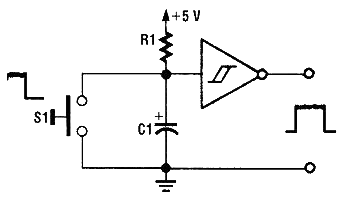
\includegraphics[width = 0.4\textwidth]{billeder/debounceSchematic.png}
	\caption{Anti debouncing kredsløb}\label{fig:antidebouncingcircuit}
\end{figure}

\section{Filter}
Filtreringen af signalet er opdelt i isolering af manchet tryk og isolering af pulserende signal. På figur \ref{fig:filterschematics} ses opdelingen af signalet i to til ADCen. Dyberer forklaring af filterdesignet kan findes under afsnit \ref{title:filters} omkring filter design.

\begin{figure}[H]
	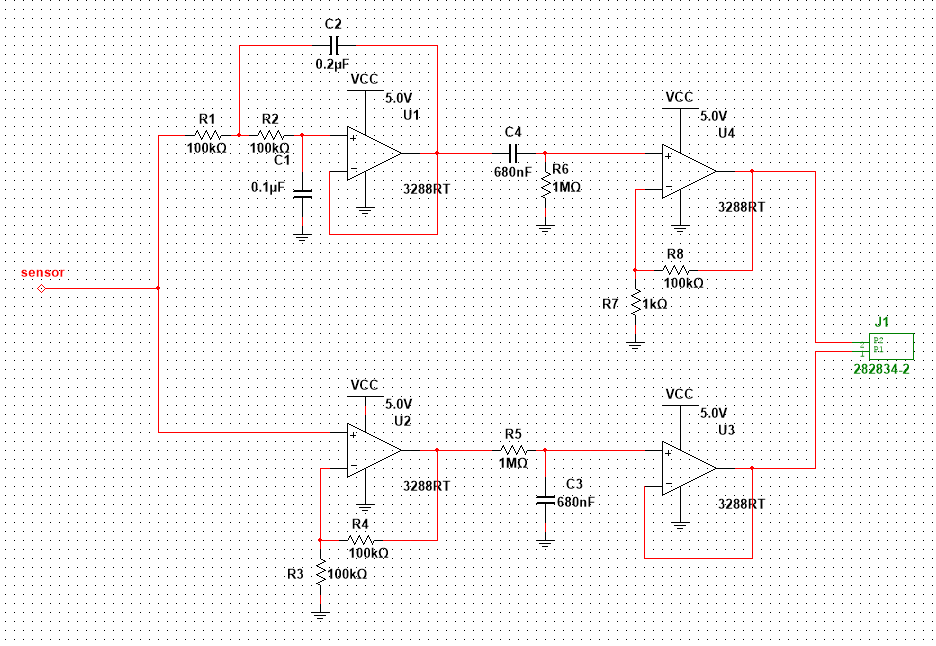
\includegraphics[width = \textwidth]{billeder/filterSchematics.png}
	\caption{Schematics over filter design}\label{fig:filterschematics}
\end{figure}

\section{Timer}
For at kunne lave tidsstempler til målinger med konditioneringsapparatet var prototypen nød til at have en real time clock, som kunne holde korrekt tid, selvom apparatet blev slukket. Dette er opnået ved hjælp af en \textit{timekeeping chip} model DS1302(Se datablad \fixme{reference til datablad DS1302}. Når prototypen er tændt forsynes den via konditioneringsapparatets strømforsyning, og når prototypen er slukket forsynes DS1302 med et knapcelle batteri. Se figur \ref{fig:timerschematic} for at se hvordan timeren er komplet på arduino. 
\begin{figure}[H]
	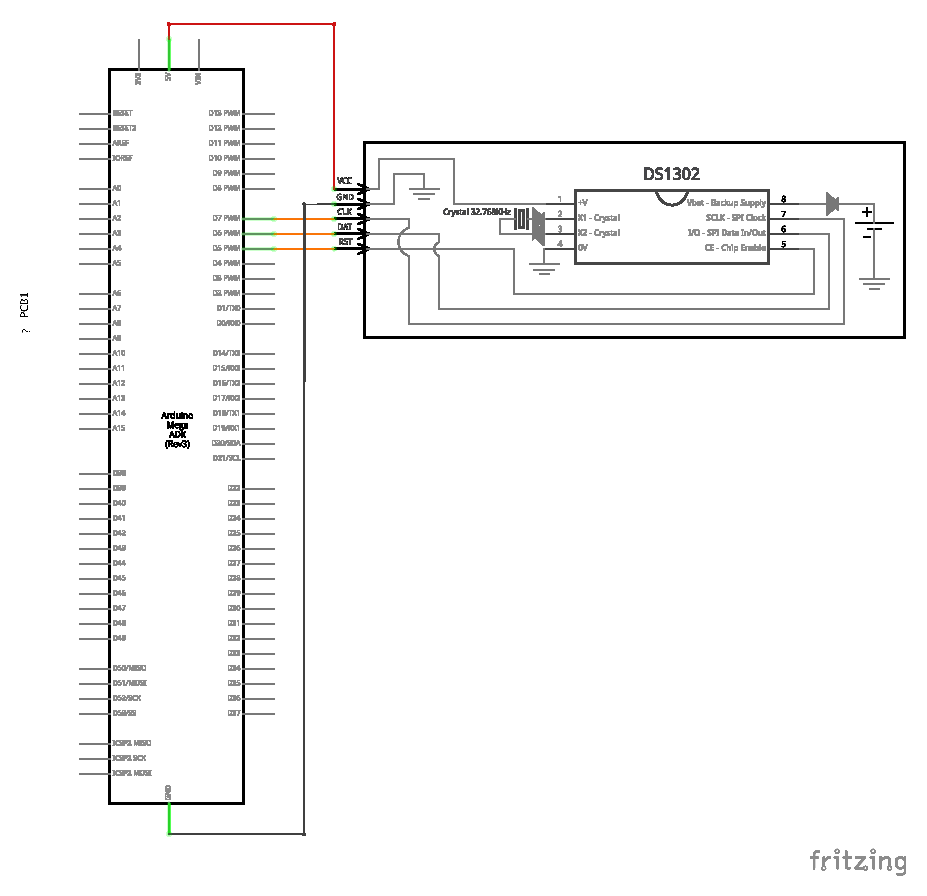
\includegraphics[trim = 15 30 0 0, clip = true, width = \textwidth]{billeder/Timer_schem.pdf}
	\caption{Oversigt over hvordan DS1302 er forbundet}\label{fig:timerschematic}
\end{figure}

\section{Display}
Til styring af bruger interfacet og feedback. Displayet er 2.2" med en opløsning på 320x240. Displayet styres med IC'en ILI9340 (Se datablad \fixme{Reference til ILI9340}). Kommunikation med displayet foregår via en SPI forbindelse som er koblet til Arduino Mega's digitale port 50, 51 og 52. For komplet interface se figur
\begin{figure}[H]
	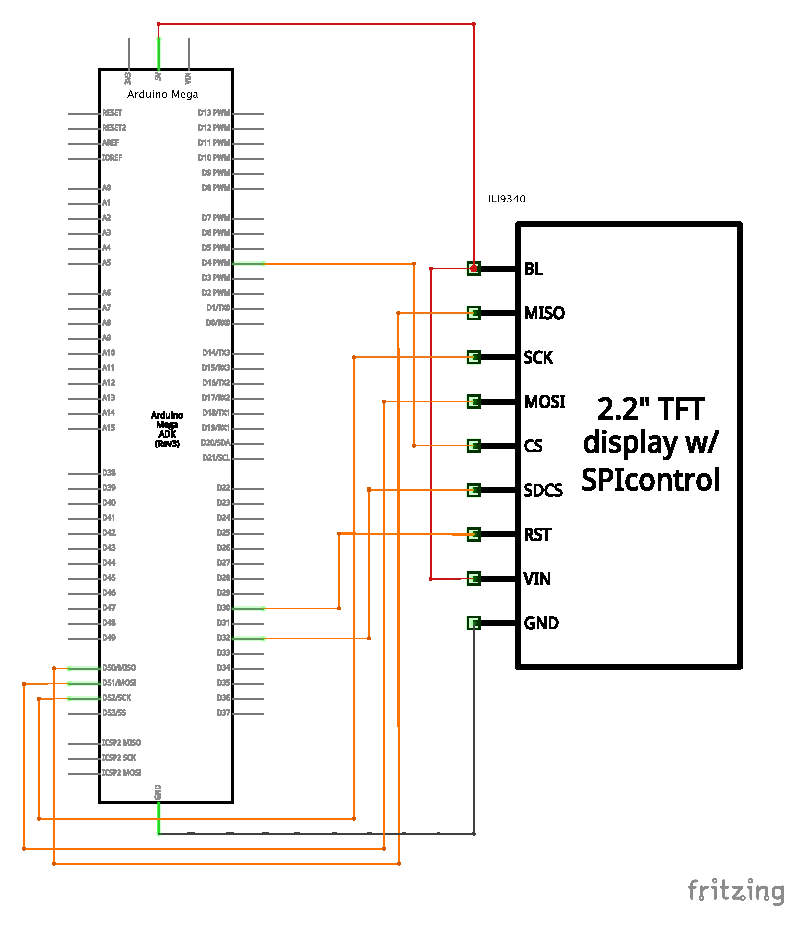
\includegraphics[trim = 10 30 0 0, clip = true, width = \textwidth]{billeder/Display_schem.pdf}
	\caption{Oversigt over hvordan ILI9340 er forbundet}\label{fig:displayschematic}
\end{figure}


\section{Motor shield}
Arduino motor shield implementerer L298P (se figur \ref{fig:shieldfront} og \ref{fig:shieldback} med selvinduktion beskyttelse og en galvanisk adskillelse af motor forsyning og den logiske strømforsyning. Schematics over boarded kan ses i bilag \fixme{reference til datablad}. Desuden er motor shield modificeret, så det har en ekstern strøm forsyning på 12V. Derfor er 5V forbindelse mellem arduino og motor shield brudt.
\begin{figure}[H]
	\begin{minipage}{0.5\textwidth}
		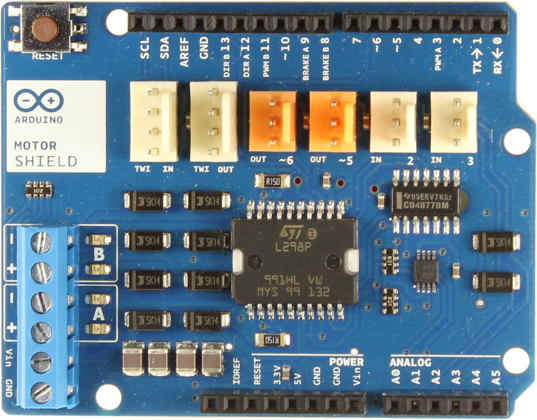
\includegraphics[width = \textwidth]{billeder/shieldforside.png}
		\caption{Arduino motorshield forside}\label{fig:shieldfront}
	\end{minipage}
	\begin{minipage}{0.5\textwidth}
		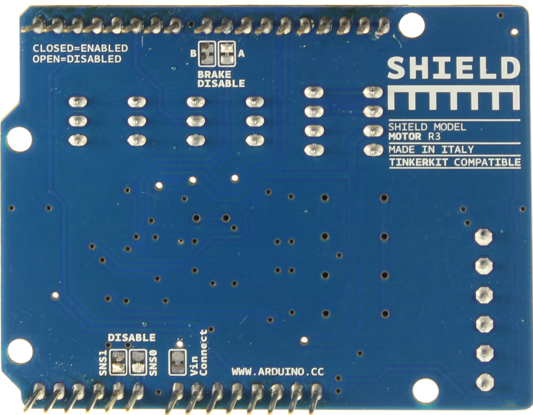
\includegraphics[width = \textwidth]{billeder/shieldbagside.png}
		\caption{Knaptryk hvor der er implementeret et anti debouncing kredsløb.}\label{fig:shieldback}
	\end{minipage}
\end{figure}